% !TEX root = morphkasten.tex

\section{Entladen}


%##############
\subsection{Kippen}
\begin{figure} [hbp]
	\centering
	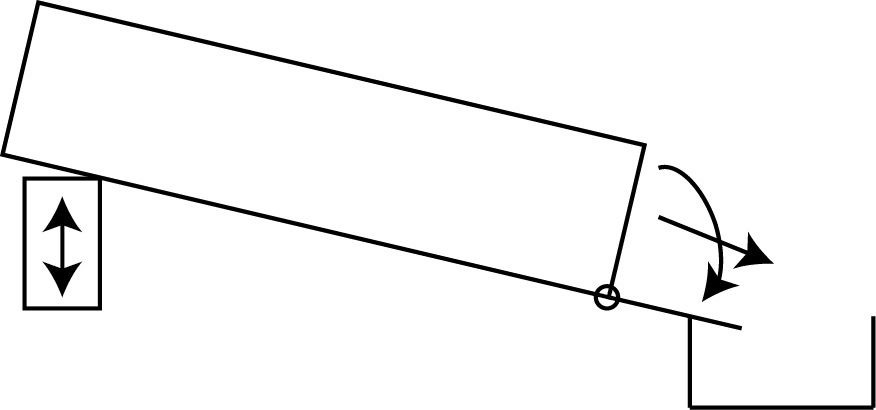
\includegraphics[width=0.7\textwidth]{fig/Entladen_Kippen.png}
	\caption{Kippen}
\end{figure}

\begin{table}[h]
\begin{tabular}{p{0.5\textwidth} | p{0.5\textwidth}}


 \textbf{Vorteile} & \textbf{Nachteile} \\ \hline
	 
\begin{itemize}
\item Kippwinkel kann eingestellt werden
\item Problemloses Abladen des Schüttgutes
\end{itemize}

 
 &
 
\begin{itemize}
\item Motor für Kippen notwendig
\item Drehgelenk an Entladebehälter notwendig
\end{itemize}

\end{tabular}
\end{table}

\begin{table}[h]
\begin{tabular}{p{0.5\textwidth}p{0.5\textwidth}}


 \textbf{Risiken} & \\ \hline
	 
\begin{itemize}
\item Unpräzises Anfahren des Abladebehälters
\end{itemize}

 
\end{tabular}
\end{table}

\pagebreak


%##############
\subsection{Schrägbehälter}

\begin{figure} [hbp]
	\centering
	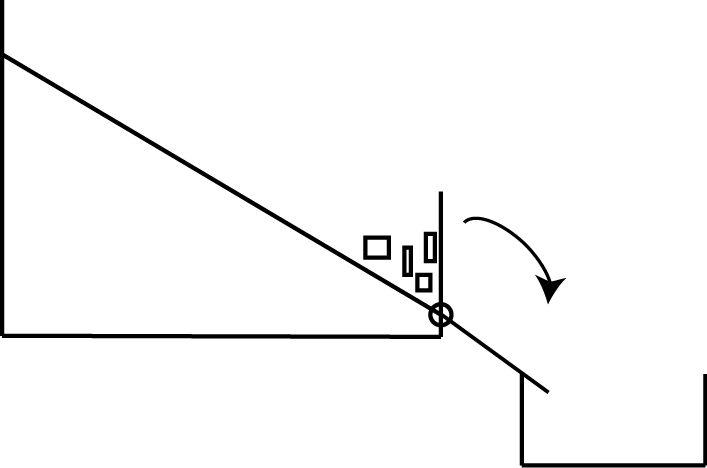
\includegraphics[width=0.5\textwidth]{fig/Entladen_Schraegbehaelter.png}
	\caption{Schrägbehälter}
\end{figure}

\begin{table}[h]
\begin{tabular}{p{0.5\textwidth} | p{0.5\textwidth}}


 \textbf{Vorteile} & \textbf{Nachteile} \\ \hline
	 
\begin{itemize}
\item Klappe öffnen als einzige Funktion
\item Einfacher Aufbau
\end{itemize}

 
 &
 
\begin{itemize}
\item Klappe muss nach Einladen noch ins Zielfeld gebracht werden
\end{itemize}

\end{tabular}
\end{table}

\begin{table}[h]
\begin{tabular}{p{0.5\textwidth}p{0.5\textwidth}}


 \textbf{Risiken} & \\ \hline
	 
\begin{itemize}
\item Nicht vollständiges Entladen
\end{itemize}

 
\end{tabular}
\end{table}

\pagebreak